\chapter{Indledning}

\section{Opgaveformulering}
I dette miniprojekt, skal der laves  en audio equalizer. Denne skal kunne justere niveauet på et indkommende lydsignal i fem forskellige frekvensbånd, der er fordelt ud over det hørbare spektrum. Der skal altså laves et lavpas filter, tre båndpas filtre og et højpas filter. 
\\ \\
Det samlede impulserespns og overføringskarakteristik skal vises i to versioner: Én hvor filtreringen foregår i sample-domænet, og én som er baseret på multiplikation af de respektive komplekse frekvensspektre. 
\\ \\
I miniprojektet skal der både forekomme FIR og IIR filter. 


\section{Audio Equalizer}
Man benytter en audio equalizer i musikbranchen. Equalization betyder udligning. Det er en proces, hvor man justere balancen mellem frekvenskomponenter inden for et elektronisk signal. 

\begin{figure}
	\centering
	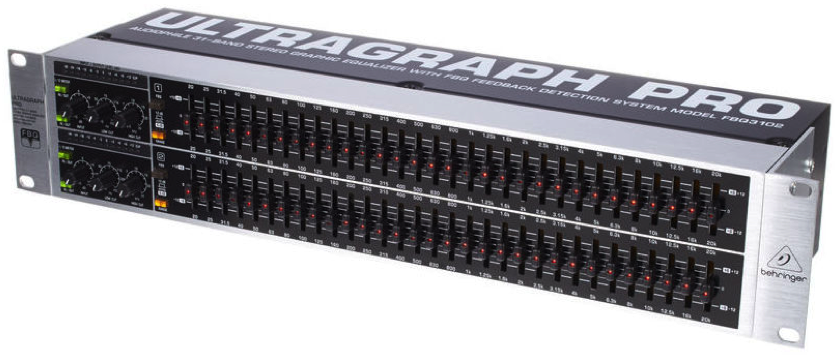
\includegraphics[width=0.6\textwidth]{Figur/Snip20151111_60}
	\caption{Equalizer}
\end{figure}

Et stereoanlæg er et eksempel på en audio aqualizer. Den har justerbare equalizere, der kan hæve eller sænke bas eller diskant frekvenser.
I et lydstudio kan man lave nogle mere detaljerede justeringer, såsom at fjerne uønskede lyde eller gøre visse instrumenter eller stemmer mere fremtrædende.
\\ \\
I dette projekt skal der som sagt laves en tilsvarende equalizer vha. LP, BP1, BP2, BP3 og HP, som enter er designet som et FIR eller IIR. 

\section{FIR}

\section{IIR}

 


